\documentclass[tikz,border=2pt]{standalone}
\usepackage{amsmath}
\usepackage{pgfplots}
\pgfplotsset{compat=1.18}
\usetikzlibrary{arrows.meta}
\begin{document}
% Example 1: f(x)=(x1-2)^2+(x2-2)^2, V={x1+x2<=2}, a=(1,1), f(a)=2; L_a is the open disc with centre (2,2) and radius sqrt2,
% which touches the line H={x1+x2=2} only at a, so H separates V and L_a and a is a global minimum on V.
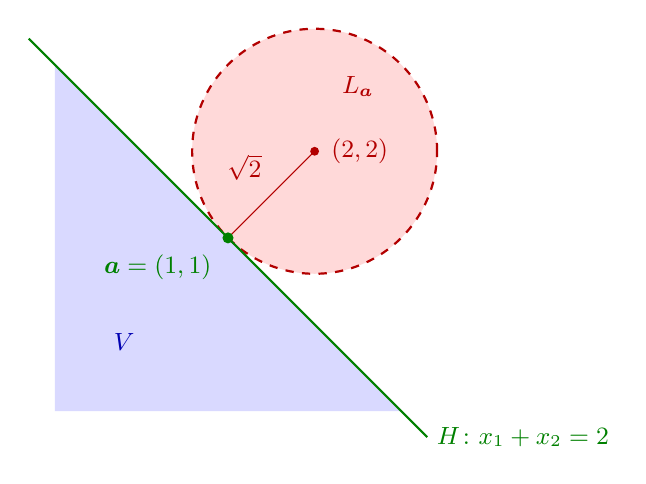
\begin{tikzpicture}[font=\small, >={Latex[length=2mm]}]
  \begin{scope}[x=1.1cm, y=1.1cm]
    \fill[blue!15] (-1,-1) -- (3,-1) -- (-1,3) -- cycle;
    \node[blue!70!black] at (-0.2,-0.2) {$V$};
    \fill[red!15] (2,2) circle ({sqrt(2)});
    \draw[red!70!black, thick, dashed] (2,2) circle ({sqrt(2)});
    \draw[green!50!black, thick] (-1.3,3.3) -- (3.3,-1.3);
    \node[green!50!black, anchor=west] at (3.3,-1.3) {$H\colon x_1+x_2=2$};
    \draw[red!70!black, thin] (2,2) -- (1,1);
    \node[red!70!black, anchor=south east] at (1.5,1.55) {$\sqrt{2}$};
    \fill[red!70!black] (2,2) circle (1.6pt);
    \node[red!70!black, anchor=west] at (2.08,2) {$(2,2)$};
    \node[red!70!black] at (2.5,2.75) {$L_{\boldsymbol{a}}$};
    \fill[green!50!black] (1,1) circle (2pt);
    \node[green!50!black, anchor=north east] at (0.92,0.92) {$\boldsymbol{a}=(1,1)$};
  \end{scope}
\end{tikzpicture}
\end{document}
